%%%%%%%%%%%%%%%%%%%%%%%%%%%%%%%%%%%%%%%%%
% Short Sectioned Assignment LaTeX Template Version 1.0 (5/5/12)
% This template has been downloaded from: http://www.LaTeXTemplates.com
% Original author:  Frits Wenneker (http://www.howtotex.com)
% License: CC BY-NC-SA 3.0 (http://creativecommons.org/licenses/by-nc-sa/3.0/)
%%%%%%%%%%%%%%%%%%%%%%%%%%%%%%%%%%%%%%%%%

% \documentclass[paper=a4, fontsize=11pt]{scrartcl} % A4 paper and 11pt font size
\documentclass[11pt, a4paper]{book}
\usepackage[T1]{fontenc} % Use 8-bit encoding that has 256 glyphs
\usepackage[utf8]{inputenc}
\usepackage{fourier} % Use the Adobe Utopia font for the document - comment this line to return to the LaTeX default
\usepackage{listings} % para insertar código con formato similar al editor
\usepackage[spanish, es-tabla]{babel} % Selecciona el español para palabras introducidas automáticamente, p.ej. "septiembre" en la fecha y especifica que se use la palabra Tabla en vez de Cuadro
\usepackage{url} % ,href} %para incluir URLs e hipervínculos dentro del texto (aunque hay que instalar href)
\usepackage{graphics,graphicx, float} %para incluir imágenes y colocarlas
\usepackage[gen]{eurosym} %para incluir el símbolo del euro
\usepackage{cite} %para incluir citas del archivo <nombre>.bib
\usepackage{enumerate}
\usepackage{hyperref}
\usepackage{graphicx}
\usepackage{tabularx}
\usepackage{booktabs}
\usepackage{longtable}
\usepackage{lscape}

\usepackage[table,xcdraw]{xcolor}
\hypersetup{
	colorlinks=true,	% false: boxed links; true: colored links
	linkcolor=black,	% color of internal links
	urlcolor=cyan		% color of external links
}
\renewcommand{\familydefault}{\sfdefault}
\usepackage{fancyhdr} % Custom headers and footers
\pagestyle{fancyplain} % Makes all pages in the document conform to the custom headers and footers
\fancyhead[L]{} % Empty left header
\fancyhead[C]{} % Empty center header
\fancyhead[R]{Daniel González Serrano} % My name
\fancyfoot[L]{} % Empty left footer
\fancyfoot[C]{} % Empty center footer
\fancyfoot[R]{\thepage} % Page numbering for right footer
%\renewcommand{\headrulewidth}{0pt} % Remove header underlines
\renewcommand{\footrulewidth}{0pt} % Remove footer underlines
\setlength{\headheight}{13.6pt} % Customize the height of the header

\usepackage{titlesec, blindtext, color}
\definecolor{gray75}{gray}{0.75}
\newcommand{\hsp}{\hspace{20pt}}
\titleformat{\chapter}[hang]{\Huge\bfseries}{\thechapter\hsp\textcolor{gray75}{|}\hsp}{0pt}{\Huge\bfseries}
\setcounter{secnumdepth}{4}
\usepackage[Lenny]{fncychap}


\begin{document}

	% Plantilla portada UGR
	\begin{titlepage}
\newlength{\centeroffset}
\setlength{\centeroffset}{-0.5\oddsidemargin}
\addtolength{\centeroffset}{0.5\evensidemargin}
\thispagestyle{empty}

\noindent\hspace*{\centeroffset}\begin{minipage}{\textwidth}

\centering

\includegraphics[width=0.9\textwidth]{logos/logo_ugr.jpg}\\[1.4cm]

\textsc{ \Large TRABAJO FIN DE GRADO\\[0.2 cm]}
\textsc{ GRADO EN INGENIERÍA INFORMÁTICA}\\[1 cm]

{\Huge\bfseries Memes para todos \\}
\noindent\rule[-1ex]{\textwidth}{3 pt}\\[3.5 ex]
{\large\bfseries Almacenamiento Online }
\end{minipage}

\vspace{2.5cm}
\noindent\hspace*{\centeroffset}
\begin{minipage}{\textwidth}
\centering

\textbf{Autor}\\ {Daniel González Serrano}\\[2.5 ex]
\textbf{Director}\\ {Juan Julián Merelo Guervós}\\[2 cm]

\includegraphics[width=0.3\textwidth]{logos/etsiit_logo.png}\\[0.1 cm]
\textsc{Escuela Técnica Superior de Ingenierías Informática y de Telecomunicación}\\
\textsc{---}\\
Granada, \today
% Mostrar nombre de mes y año de entrega del documento

\end{minipage}
\end{titlepage}


	% Plantilla prefacio UGR
	\thispagestyle{empty}

\begin{center}
{\large\bfseries Memes para todos \\ Almacenamiento Online }\\
\end{center}
\begin{center}
Daniel González Serrano\\
\end{center}

%\vspace{0.7cm}

\vspace{0.5cm}
\noindent\textbf{Palabras clave}: \textit{software libre}
\vspace{0.7cm}

\noindent\textbf{Resumen}\\
	

\cleardoublepage

\begin{center}
	{\large\bfseries Igual, pero en inglés}\\
\end{center}
\begin{center}
	Daniel González Serrano\\
\end{center}
\vspace{0.5cm}
\noindent\textbf{Keywords}: \textit{open source}, \textit{floss}
\vspace{0.7cm}

\noindent\textbf{Abstract}\\


\cleardoublepage

\thispagestyle{empty}

\noindent\rule[-1ex]{\textwidth}{2pt}\\[4.5ex]

D. \textbf{Juan Julián Merelo Guervós}, Profesor(a) del ...

\vspace{0.5cm}

\textbf{Informo:}

\vspace{0.5cm}

Que el presente trabajo, titulado \textit{\textbf{Chief}},
ha sido realizado bajo mi supervisión por \textbf{Estudiante}, y autorizo la defensa de dicho trabajo ante el tribunal
que corresponda.

\vspace{0.5cm}

Y para que conste, expiden y firman el presente informe en Granada a \today

\vspace{1cm}

\textbf{El/la director(a)/es: }

\vspace{5cm}

\noindent \textbf{(nombre completo tutor/a/es)}

\chapter*{Agradecimientos}






	% Índice de contenidos
	\newpage
	\tableofcontents

	% Índice de imágenes y tablas
	\newpage
	\listoffigures

	% Si hay suficientes se incluirá dicho índice
	\listoftables 
	\newpage

  % Introducción 
	\chapter{Introducción}

¿Alguna vez ha tenido problemas a la hora de encontrar una imagen en su galería?

Si la respuesta es sí y que después de estar guardando contenido en su solución de almacenamiento elegida durante un tiempo, se vuelve insostenible y ya no es nada útil, el problema que se propone resolver este TFG le va a ser de interés. Al igual que usted, hay mucha gente que, debido a la gran cantidad de contenido digital que maneja le es imposible realizar una acción tan fácil (o difícil) como es la de encontrar una imagen.

\section{Contexto y motivación}

En este escenario de generación de contenido digital sin parangón se presenta un desafío para los creadores de contenido: la gestión y almacenamiento eficiente, eficaz
y ágil de dicho contenido. A pesar de contar con diversas plataformas de almacenamiento en la nube y soluciones de gestión de contenidos digitales, la mayoría de
estas soluciones tienen diferentes limitaciones que afectan a la organización, ordenación y accesibilidad de este contenido. La necesidad de una solución que permita
a los usuarios almacenar, organizar y acceder a su amplio repertorio contenido digital de forma eficiente, eficaz y ágil es evidente.

Esta falta de soluciones eficientes, eficaces y ágiles para la gestión y almacenamiento de contenido digital es la motivación principal de este proyecto. Aquí se
presenta una oportunidad significativa para desarrollar un sistema más robusto y adaptado a las necesidades actuales.

Al mejorar la eficiencia, eficacia y agilidad a la hora de la gestión y almacenamiento del contenido digital los usuarios pueden dedicarse a lo que realmente les importa:
la creación de contenido permitiéndoles así dedicarle más tiempo a la creatividad y a la expresión que requiere la creación de contenido digital sin miedo a perder o
no poder acceder a su contenido.

En este contexto y motivación, el presente proyecto se propone abordar estas limitaciones, diseñando y desarrollando un sistema de almacenamiento online que no solo almacene, 
sino que también organice, ordene y facilite el acceso a contenido digital de manera intuitiva y eficiente.

\section{Definición del problema}

Como se ha señalado previamente, la generación masiva de contenido digital ha creado un problema de gestión y almacenamiento del mismo. A pesar de la existencia de
soluciones en la nube y plataformas de gestión de contenido, existen limitaciones a la hora de la gestión y organización de imágenes. La ausencia de una solución que
permita la gestión y organización de imágenes de forma centralizada y eficiente es el problema que se pretende abordar con este proyecto.

    \subsection{Usuarios identificados}

    \begin{itemize}
        \item \textbf{Nombre}: María Rodríguez.
        \item \textbf{Edad}: 30 años.
        \item \textbf{Educación}: Licenciada en comunicación digital.
        \item \textbf{Ocupación}: Creadora de contenido.
        \item \textbf{Conocimientos y actitud hacia la tecnología}: Tiene conocimientos avanzados en herramientas digitales y plataformas de creación de contenido. Es entusiasta y proactiva hacia las nuevas tecnologías, siempre dispuesta a explorar nuevas soluciones que mejoren su experiencia y flujo de trabajo a la hora de la creación y gestión de contenido digital.
        \item \textbf{Dispositivos}:
            \begin{itemize}

            \item \textbf{¿Cuáles usa?}: Ordenador portátil de última generación, teléfono móvil de última generación y tablet.
            \item \textbf{¿Cuándo los usa?}: Durante todo el día.
            \item \textbf{¿Para qué los usa?}: Para mantenerse al tanto de las tendencias, interactuar con su audiencia y crear contenido.

            \end{itemize}
        \item \textbf{Misión}:
        \item 
            \begin{itemize}

                \item \textbf{¿Utilizaría nuestra aplicación?}: Sí.

                \item \textbf{¿Qué le gustaría que tuviera?}: Un sistema de almacenamiento en la nube que le permita subir y organizar fácilmente su contenido desde cualquier lugar. Le gustaría tener un acceso rápido y sencillo desde cualquier dispositivo con conexión a Internet, una interfaz intuitiva, un sistema de gestión de versiones, seguridad y privacidad, un sistema de búsqueda avanzada que permita encontrar cualquier contenido.

            \end{itemize}
        
    \end{itemize}

    \begin{itemize}
        \item \textbf{Nombre}: Juan Pérez.
        \item \textbf{Edad}: 40 años.
        \item \textbf{Educación}: Ingeniero de Sistemas.
        \item \textbf{Ocupación}: CTO.
        \item \textbf{Conocimientos y actitud hacia la tecnología}: Conocimientos avanzados en sistemas y tecnologías. Actitud positiva y pragmática.
        \item \textbf{Dispositivos}:
            \begin{itemize}
            \item \textbf{¿Cuáles usa?}: Ordenador de sobremesa y teléfono móvil. 
            \item \textbf{¿Cuándo los usa?}: Principalmente durante las horas laborales.
            \item \textbf{¿Para qué los usa?}: Para trabajar, informarse y comunicarse.
            \end{itemize}
        \item \textbf{Misión}:
            \begin{itemize}

                \item \textbf{¿Utilizaría nuestra aplicación?}: No. Prefiere un almacenamiento local, no considera necesario un sistema complejo y desconfía de la nube. Utiliza Microsoft OneDrive que ya le brinda la flexibilidad de acceso a los archivos, seguridad, privacidad y el sistema de búsqueda y gestión.

                \item \textbf{¿Qué le gustaría que tuviera?}: Le gustaría que no tuviera complicaciones a la hora de la instalación y configuración. Todas las facilidades que ya le brinda Microsoft OneDrive más alguna característica única e interesante para él.

            \end{itemize}
        
    \end{itemize}

    \begin{itemize}
        \item \textbf{Nombre}: Laura Martínez.
        \item \textbf{Edad}: 35 años.
        \item \textbf{Educación}: Licenciada en Bellas Artes.
        \item \textbf{Ocupación}: Fotógrafa profesional.
        \item \textbf{Conocimientos y actitud hacia la tecnología}: Tiene conocimientos avanzados en técnicas fotográficas y edición de imágenes. Prefiere soluciones sencillas y fáciles de usar. No le gusta perder el tiempo en configuraciones y opciones complejas.
        \item \textbf{Dispositivos}:
            \begin{itemize}

            \item \textbf{¿Cuáles usa?}: Ordenador portátil de alta gama y dispositivo móvil inteligente.
            \item \textbf{¿Cuándo los usa?}: Durante todo el día.
            \item \textbf{¿Para qué los usa?}: Revisar correos, redes sociales además de editar y visualizar imágenes.

            \end{itemize}
        \item \textbf{Misión}:
        \item 
            \begin{itemize}

                \item \textbf{¿Utilizaría nuestra aplicación?}: No. Siempre ha experimentado una pérdida de calidad al subir su contenido a la nube. Prefiere tener un almacenamiento local como el NAS que tiene para almacenar y organizar su contenido.

                \item \textbf{¿Qué le gustaría que tuviera?}: Su sistema idea es un sistema que facilite la organización, gestión y almacenamiento de su contenido de forma intuitiva, simple y eficaz sin pérdidas de calidad.

            \end{itemize}
        
    \end{itemize}

    \begin{itemize}
        \item \textbf{Nombre}: Carlos Sánchez
        \item \textbf{Edad}: 45 años.
        \item \textbf{Educación}: Licenciado en administración de empresas.
        \item \textbf{Ocupación}: Dueño de un pequeño negocio.
        \item \textbf{Conocimientos y actitud hacia la tecnología}: Conocimientos muy básicos en tecnología. Utiliza la tecnología para ganar difusión en su negocio aunque no sea un experto. Actitud conservadora y pragmática.
        \item \textbf{Dispositivos}:
            \begin{itemize}

            \item \textbf{¿Cuáles usa?}: Ordenador de sobremesa y teléfono inteligente.
            \item \textbf{¿Cuándo los usa?}: Durante las horas laborales.
            \item \textbf{¿Para qué los usa?}: Para atender llamadas y mensajes de clientes, comprobar el correo, redes sociales y gestionar su negocio.

            \end{itemize}
        \item \textbf{Misión}:
        \item 
            \begin{itemize}

                \item \textbf{¿Utilizaría nuestra aplicación?}: Sí, pero al tener una conexión inestable (a veces no funciona Internet) duda de si es una buena solución para él.

                \item \textbf{¿Qué le gustaría que tuviera?}: Valoraría mucho que el sistema ofreciera opciones de gestión offline y que no dependa de tener una conexión estable a Internet además de que fuera fácil de implementar y usar.

            \end{itemize}
        
    \end{itemize}

    \begin{itemize}
        \item \textbf{Nombre}: Marta González.
        \item \textbf{Edad}: 28 años.
        \item \textbf{Educación}: Graduada en Diseño Multimedia.
        \item \textbf{Ocupación}: Diseñadora Autónoma.
        \item \textbf{Conocimientos y actitud hacia la tecnología}: Tiene conocimientos avanzados en software de diseño gráfico y multimedia. Tiene una actitud positiva hacia la tecnología para mejorar su eficiencia en la organización y archivos digitales.
        \item \textbf{Dispositivos}:
            \begin{itemize}

            \item \textbf{¿Cuáles usa?}: Ordenador de sobremesa potente, teléfono inteligente y tableta gráfica.
            \item \textbf{¿Cuándo los usa?}: Durante las horas diurnas pero también algunas veces por la noche.
            \item \textbf{¿Para qué los usa?}: Para realizar sus proyectos de ilustración y diseño.

            \end{itemize}
        \item \textbf{Misión}:
        \item 
            \begin{itemize}

                \item \textbf{¿Utilizaría nuestra aplicación?}: Sí. Aunque siempre que ha utilizado un sistema para la organización de contenido ha tenido problemas cuando la cantidad del mismo es muy grande.

                \item \textbf{¿Qué le gustaría que tuviera?}: Le gustaría que fuera realmente escalable y mantenible aun con cantidades grandes de contenido.

            \end{itemize}
        
    \end{itemize}


\section{Historias de usuario}

\subsection{María Rodríguez (Creadora de contenido)}

\begin{enumerate}
    \item Como María Rodríguez, quiero poder acceder a la aplicación desde mi ordenador portátil, teléfono móvil y tablet en cualquier momento.
    \item Como María Rodríguez, quiero que la interfaz sea intuitiva que me permita navegar y gestionar mi galería de memes de forma rápida y sencilla, así no tengo que dedicar mucho tiempo a aprender a manejarla.
    \item Como María Rodríguez, quiero que mi galería de memes esté protegida para que no me roben contenido.
    \item Como María Rodríguez, me gustaría que existiera la posibilidad de volver recuperar la versión anterior de algún meme.
    \item Como María Rodríguez, necesito algún tipo de búsqueda avanzada para encontrar cualquier meme ya sea por título, etiquetas o contenido del propio meme.
\end{enumerate}

\subsection{Juan Pérez (CTO)}

    \begin{enumerate}
        \item Como Juan Pérez, quiero que la instalación y configuración se puedan hacer de manera sencilla y sin complicaciones.
        \item Como Juan Pérez, quiero que existan medidas de protección como lo hace Microsoft OneDrive.
        \item Como Juan Pérez, quiero que exista la posibilidad de disponer de una herramienta para crear memes de manera rápida y sencilla.
        \item Como Juan Pérez, quiero que la gestión de los memes se haga del modo más eficiente y rápida posible así los puedo encontrar más rápido.
    \end{enumerate}

\subsection{Laura Martínez (Fotógrafa Profesional)}

    \begin{enumerate}
        \item Como Laura Martínez, quiero un sistema de almacenamiento local como el NAS que ya tengo instalado que me permita mantener la calidad de mis imágenes y evitar la pérdida de calidad.
    \end{enumerate}

\subsection{Carlos Sánchez (Dueño de un pequeño negocio)}

    \begin{enumerate}
        \item Como Carlos Sánchez, prefiero una solución que ofrezca opciones de gestión aun sin conexión a internet.
        \item Como Carlos Sánchez, necesito una solución que ofrezca opciones de edición de memes aun sin conexión a internet.
        \item Como Carlos Sánchez, quiero que se permita compartir los memes fácilmente con las diferentes redes sociales para que tenga la opción de subir en cualquier momento cualquier meme relacionado con mi negocio para ganar popularidad.
        \item Como Carlos Sánchez, quiero poder acceder desde mi móvil y ordenador personal para, por ejemplo, crear y editar los memes en el ordenador personal y luego en el móvil subirlo a RRSS.
    \end{enumerate}

\subsection{Marta González (Diseñadora Freelancer)}

    \begin{enumerate}
        \item Como Marta González, quiero que sea fácil de mantener a medida que mi colección de memes crece.
        \item Como Marta González, me gustaría que la aplicación ofreciera integraciones con otras herramientas de diseño gráfico para facilitar la importación y exportación de contenido y poder conectar varias plataformas, aplicaciones, etc.
        \item Como Marta González, valoro mucho que se puedan manejar grandes cantidades de memes sin experimentar problemas de rendimiento o dificultades en la organización u ordenación.
    \end{enumerate}

\section{Objetivos}

La esencia de los objetivos radica en diseñar y desarrollar un sistema de almacenamiento en la nube. Este sistema se enfoca en resolver los diferentes problemas
identificados durante el análisis del problema. 

La experiencia de usuario es un pilar fundamental de nuestro proyecto. Varios de los problemas y de las personas identificadas en el análisis del problema
pueden resolverse con una útil, accesible, intuitiva y simple interfaz de usuario reduciendo los clics necesarios y disminuyendo el tiempo de carga,
todo con el objetivo de aumentar la satisfacción del usuario.

La gestión, ordenación y organización del contenido digital del usuario debe ser nuestro principal objetivo. Todo esto para reducir el tiempo que el usuario
dedica a la gestión de su contenido y aumentar el tiempo que dedica a la creación de contenido.

La compatibilidad con diferentes dispositivos y sistemas operativos es otro de los objetivos de este proyecto. El usuario debe poder acceder a su contenido
desde cualquier dispositivo con conexión a Internet y con cualquier sistema operativo.

La seguridad y privacidad del contenido del usuario es otro de los objetivos de este proyecto. El usuario debe poder confiar en el sistema de almacenamiento
y no debe preocuparse por la seguridad y privacidad de su contenido.

Además de estos objetivos existen otros como la incorporación de gestión de versiones para mejorar la experiencia del usuario y la implementación de un sistema
de búsqueda avanzada que permita al usuario encontrar cualquier contenido de forma rápida y sencilla.

Finalmente, otro objetivo de este proyecto es relativo a la evaluación y validación del sistema por parte del cliente, que, en nuestro caso es el tutor
y el tribunal. El sistema debe ser evaluado y validado por el cliente para comprobar que cumple con los requisitos y objetivos establecidos.

	% Descripción del problema y hasta donde se llega
	\chapter{Descripción del problema}



	% Estado del arte
	% 	1. Crítica al estado del arte
	% 	2. Propuesta
	\chapter{Estado del arte}

En este capítulo se revisarán las herramientas y plataformas actuales que abordan funcionalidades relacionadas con la gestión, almacenamiento y edición colaborativa de memes. Esta revisión permitirá identificar los valores y limitaciones de las soluciones existentes frente a la propuesta de este proyecto.

Vamos a dividir este apartado en dos secciones: la primera sección que se centrará en la comparación con plataformas de creación y edición de memes y la segunda sección que se centrará en la comparación con plataformas de almacenamiento de contenido gráfico.

\section{Herramientas para la Creación y Edición de Memes}

Actualmente, existen diversas aplicaciones enfocadas en la creación y edición de memes, cada una con características específicas en cuanto a funcionalidad, facilidad de uso y accesibilidad. A continuación, se describen algunas de las herramientas más populares y sus características:

\begin{itemize}
  \item \textbf{Generación y creación de memes:} aplicaciones como \textit{\textbf{\href{https://imgflip.com/memegenerator}{Meme Generator de imgflip}}} y \textit{\textbf{\href{https://www.mematic.com/}{Mematic}}} permiten a los usuarios crear memes de forma rápida utilizando plantillas populares y ofreciendo opciones básicas de edición, como agregar texto y recortar imágenes. Sin embargo, estas aplicaciones presentan limitaciones cuando se requiere de una personalización más avanzada o colaboración. Además, la falta de opciones de almacenamiento organizado reduce su utilidad para quienes desean reutilizar y categorizar memes.
  \item \textbf{Aplicaciones orientadas a la edición online:} Plataformas como \href{https://www.canva.com/es_es/}{Canva} y \href{https://www.photopea.com/}{Photopea} permiten la edición de imágenes con mayores posibilidades de personalización y funciones avanzadas de edición gráfica. No obstante, estas herramientas suelen tener una curva de aprendizaje más alta, ya que están diseñadas para una gama más amplia de trabajos de diseño gráfico. A mayores, la colaboración y la organización de memes en colecciones no son características comunes en estas plataformas.
  \item \textbf{Aplicaciones con enfoque social:} redes sociales como \href{https://www.instagram.com/}{Instagram} permiten a los usuarios generar contenido visual con opciones para añadir texto y stickers, lo cual puede ser utilizado para crear memes. Sin embargo, estas plataformas no están diseñadas para la gestión centralizada de memes y carecen de una estructura adecuada para la categorización o reutilización de contenido, limitando su efectividad para un uso colaborativo o profesional.
\end{itemize}

\section{Plataformas de almacenamiento y organización de contenido visual}

La organización y almacenamiento centralizado es un aspecto clave para este proyecto, especialmente para usuarios que producen contenido de forma recurrente. En el mercado actual existen plataformas de almacenamiento de imágenes, pero ninguna está específicamente orientada a la gestión y reutilización de memes. Las plataformas destacadas incluyen:

\begin{itemize}
  \item \textbf{\href{https://www.google.com/intl/es_es/photos/about/}{Google Photos}} Esta plataformas de almacenamiento en la nube permiten a los usuarios organizar sus archivos visuales mediante etiquetas y carpetas. A pesar de su popularidad, carece de funcionalidades específicas para la gestión de memes, como plantillas reutilizables y sistemas de búsqueda avanzada que consideren categorías de memes o contextos humorísticos.
  \item \textbf{\href{https://www.icloud.com/}{iCloud}}, \textbf{\href{https://drive.google.com/drive/my-drive?hl=es-419}{Google Drive}}, \textbf{\href{https://mega.io/es}{Mega}}, \textbf{\href{https://www.microsoft.com/es-es/microsoft-365/onedrive/online-cloud-storage}{OneDrive}} y \textbf{\href{https://www.dropbox.com/}{Dropbox}} son opciones de almacenamiento con funcionalidades completas, aunque ninguna ofrece herramientas especializadas para la gestión y organización de memes. ICloud destaca por su integración en el ecosistema de Apple, permitiendo sincronizar archivos entre dispositivos de la marca. Google Drive y OneDrive, de Google y Microsoft respectivamente, ofrecen un acceso sencillo y compartido a los archivos en la nube. Mega y Dropbox se diferencian al proporcionar una mayor capacidad de almacenamiento gratuito. Sin embargo, en todos los casos, estas plataformas se enfocan en el almacenamiento general de archivos sin opciones específicas para memes.
  \item \textbf{\href{https://nextcloud.com/es/}{Nextcloud}:} Ofrece opciones avanzadas de sincronización y colaboración en la nube, adaptándose parcialmente a la gestión de memes. Sin embargo, su configuración y administración pueden ser complicadas para usuarios sin conocimientos técnicos. Además, carece de herramientas específicas para la edición o categorización de memes, limitando su utilidad como herramienta especializada.
  \item \textbf{\href{https://es.pinterest.com/}{Pinterest}:} Aunque no es una plataforma de almacenamiento en el sentido tradicional, Pinterest permite a los usuarios organizar contenido visual en tableros categorizados, lo cual facilita la agrupación de memes por temas. Sin embargo, no ofrece herramientas para la edición directa de memes, y su estructura no está orientada al almacenamiento profesional o colaborativo de este tipo de contenido.
\end{itemize}

\section{Conclusión de comparativas}

En esta comparación de alternativas con el proyecto, se destacan varios puntos diferenciadores que consolidan esta propuesta como una solución \textbf{innovadora}:

\begin{itemize}
  \item \textbf{Facilidad de acceso y colaboración:} Al ser una aplicación web permite a los usuarios acceder desde cualquier dispositivo y colaborar en la creación y modificación de memes, algo que no ofrecen muchas de las plataformas revisadas.
  \item \textbf{Centralización y organización:} La plataforma incorpora un sistema específico para el almacenamiento y organización de memes en catálogos, incluyendo funcionalidades avanzadas de búsqueda y gestión de plantillas reutilizables. Esto representa una ventaja significativa frente a las soluciones actuales de almacenamiento general.
  \item \textbf{Especialización en memes:} A diferencia de las herramientas de edición de imágenes o plataformas de almacenamiento genéricas, esta aplicación se enfoca principalmente en la creación y gestión de memes. Esto permite una optimización de la experiencia del usuario y la personalización de herramientas específicas para este tipo de contenido, sin limitar la posibilidad de que se suba y organice otro tipo de material visual. Esto asegura que, aunque centrada en los memes, la plataforma sea versátil y pueda adaptarse a otras necesidades de los usuarios.
\end{itemize}
	
	\chapter{Planificación}

Como ya se ha mencionado, el proyecto seguirá las prácticas y principios del enfoque ágil, que se fundamenta en los 17 principios delineados en \href{https://agilemanifesto.org/iso/es/manifesto.html}{el manifiesto ágil}. Ágil no es una metodología ni un marco de trabajo, sino una mentalidad que permite a las organizaciones ser más receptivas al cambio. Estos principios están diseñados para asegurar la satisfacción del cliente a través de la entrega temprana y continua de valor, con un fuerte enfoque en la excelencia técnica, el buen diseño, la planificación y la simplicidad.

Estos principios no son solo una referencia teórica, sino que se han aplicado con éxito en proyectos reales y actuales, de acuerdo con~\cite{berlas2024software}. Este informe presenta una revisión completa de la investigación publicada sobre las métricas de software en el desarrollo ágil y resalta su efectividad en diversos contextos, incluyendo pequeñas y medianas empresas.

\begin{itemize}
    \item \textbf{¿Se está usando enfoques ágiles?} El informe indica que los enfoques ágiles son ampliamente utilizados en la industria del software, permitiendo a los equipos de desarrollo trabajar iterativamente y responder rápidamente a las necesidades del cliente.
    \item \textbf{¿Esto verdaderamente funciona?} Según el informe, los enfoques ágiles han demostrado ser eficaces en diversos tipos de proyectos a cualquier escala proporcionando beneficios como la reducción del tiempo de comercialización, mayor satisfacción del cliente y disminución de los costos de desarrollo.
\end{itemize}    

Para garantizar la aplicación coherente de estos principios, la memoria debe desarrollarse de forma iterativa e incremental, con actualizaciones a medida que avanza el proyecto y se toman decisiones. Esto nos permite evaluar continuamente cómo estamos añadiendo valor al proyecto.

En este punto, es dónde las historias de usuario y los objetivos iniciales se convierten en la guía para el desarrollo del proyecto. Las mismas también forman parte de la planificación, pues, son las que garantizan la entrega y calidad continua de un producto.

\section{Entrega y calidad continua}

Para asegurar la calidad del proyecto y la entrega continua, se han empleado una serie de herramientas y enfoques que se han integrado en el flujo de trabajo tanto local como remoto.

La documentación del proyecto es una de las partes más importantes (junto con el código) del trabajo de fin de grado si no la que más por lo que se ha de poner especial atención en que esta sea de calidad y cumpla con los requisitos establecidos por tutor y tribunal. Para dar cuenta de esto, la memoria se ha elaborado en \href{https://www.latex-project.org/}{\LaTeX{}} que es un sistema de composición tipográfica de alta calidad; incluye funciones diseñadas para la producción de documentación técnica y científica además de estar disponible como software libre.

Para complementar, comprobar y mejorar la calidad de la documentación se han usado una serie de herramientas que se han integrado en el flujo de trabajo local tanto con extensiones de (\href{https://code.visualstudio.com/}{\textit{Visual Studio Code}}) como con herramientas ejecutadas en la línea de comandos.

En cuanto a flujos de trabajo remotos en \textit{GitHub} se han implementado uno específico para la memoria. Este flujo de trabajo se activa en cada push y se encarga de realizar verificaciones gramaticales y ortográficas con \href{https://github.com/sylvainhalle/textidote}{\textit{TeXtidote}} de la cual se sube un informe y si pasa estas verificaciones de forma satisfactoria se sube la memoria compilada en formato PDF a modo de artefacto. Este flujo de trabajo remoto junto con el local garantizan la calidad de la documentación.

Ese artefacto generado tras acabar cada \textit{milestone} o hito podría ser perfectamente entregable a un cliente final a modo de entrega continua para que vea el progreso del proyecto. A mayores, hacemos referencia al tercer principio del \href{https://agilemanifesto.org/iso/es/principles.html}{manifiesto ágil} que dice: \textit{``Entregar software funcional frecuentemente, entre dos semanas y dos meses, con preferencia al periodo de tiempo más corto''}. Además, los flujos de trabajo remotos (en \textit{GitHub}) y locales promueven el noveno principio que hace referencia a la atención continua a la excelencia técnica y el buen diseño.

\section{Metodologías para el seguimiento del desarrollo}

En esta sección se documentarán las metodologías empleadas para el seguimiento del desarrollo del proyecto. Al aplicar estas metodologías se ha conseguido una mayor eficiencia en la gestión del tiempo y de los recursos, así como una mayor calidad en la documentación y en el código fuente. Además, se explicarán las herramientas utilizadas para el control de versiones y el alojamiento del repositorio remoto del proyecto.

\subsection{\textit{Git y GitHub}: control de versiones y colaboración}

Para el control de versiones se ha empleado \textit{git} que es un sistema de control de versiones que permite llevar un control de los cambios en el código fuente.

Para la colaboración y hospedaje del código fuente se ha hecho en \textit{GitHub}, una plataforma que permite alojar proyectos de \textit{software} y colaborar en ellos. En \textit{GitHub} tenemos diferentes funcionalidades que han sido de ayuda para el desarrollo del proyecto.

\textbf{El repositorio del proyecto se puede encontrar en la siguiente dirección: \url{https://github.com/danigonzser/proyecto-tfg}.}

La transparencia y accesibilidad de GitHub facilitan la comunicación constante y la colaboración del equipo, apoyando los principios ágiles de la colaboración diaria entre desarrolladores y clientes, y de la construcción de proyectos en torno a individuos motivados.

En GitHub se integran diferentes herramientas que permiten llevar un control del desarrollo del proyecto. A continuación, se describen algunas de las funcionalidades más importantes.

\subsubsection{\textit{Issues}}

A lo largo del proyecto se van a ir encontrando diferentes problemas que se han de resolver. Para llevar un control de los mismos se han ido creando \textit{issues}. Estos no solo son descripciones de los problemas que se quieren resolver, sino que pueden ser una buena medida para saber si se progresa hacia el \textit{milestone} o no.

\begin{figure}[H]
    \caption{Captura de pantalla del listado de \textit{issues} del repositorio del proyecto de \textit{GitHub}.}
    \centering
    \vspace*{0.5cm}
    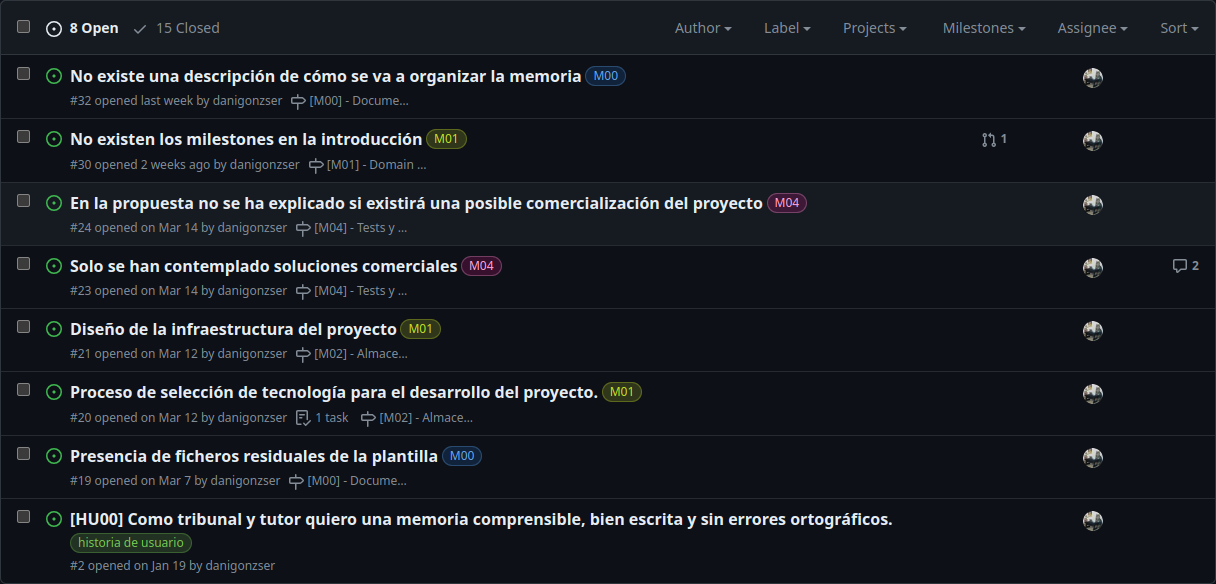
\includegraphics[scale=0.2]{figuras/github_issues.png}
\end{figure}

Existe un acceso a la documentación de la metodología seguida que se puede consultar en el siguiente \href{https://github.com/danigonzser/proyecto-tfg/issues?q=is%3Aissue+is%3Aclosed}{enlace}, aquí se encuentra el registro completo de los \textit{issues} cerrados, que ilustran el proceso de resolución de problemas y la evolución del proyecto. A continuación, se muestra un pantallazo de los \textit{issues} cerrados:

\begin{figure}[H]
    \caption{Pantallazo del listado de issues cerradas.}
    \centering
    \vspace*{0.5cm}
    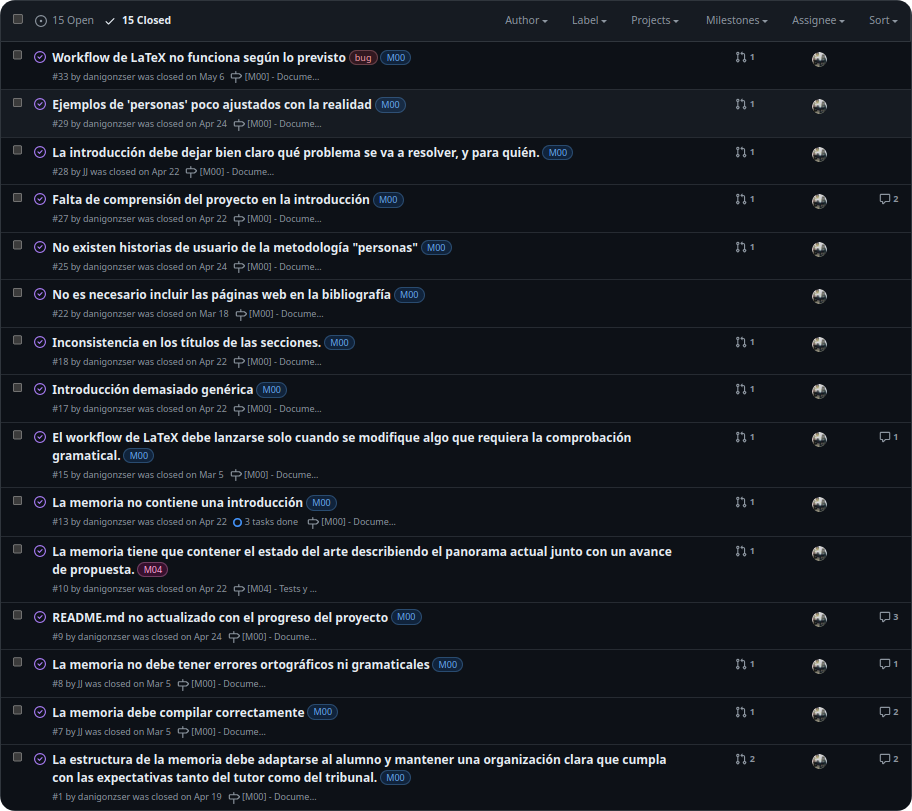
\includegraphics[scale=0.2]{figuras/listado_issues_cerradas.png}\label{fig:figuras/listado_issues_cerradas.png}
\end{figure}

\subsubsection{Pull requests}

Los pull requests son una forma de proponer cambios en el código fuente sin que estos se apliquen directamente al código fuente o rama principal sin una aprobación previa. Estos son una manera de revisar que los cambios mantengan la excelencia técnica y calidad del proyecto apoyando al noveno principio del manifiesto ágil.

Para proteger la rama principal o \textit{master} de cambios no deseados se han configurado una serie de reglas que impiden la integración de cambios a menos que:

\begin{itemize}
    \item Los tests deben de haberse realizado de manera exitosa.
    \item Que la rama esté actualizada.
    \item Que las conversaciones hayan sido resueltas.
\end{itemize}

A continuación se muestra una captura de pantalla de la lista de \textit{pull requests} del proyecto hasta el momento.

\begin{figure}[H]
    \caption{Captura de pantalla del listado de \textit{pull requests} del repositorio del proyecto de \textit{GitHub}.}
    \centering
    \vspace*{0.5cm}
    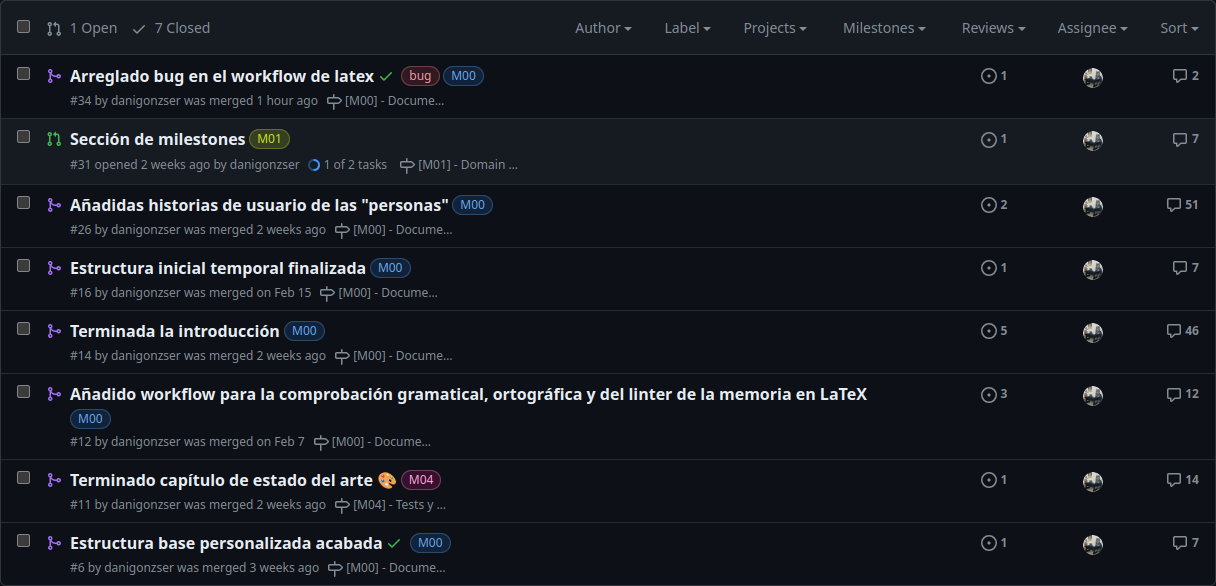
\includegraphics[scale=0.2]{figuras/listado_pull_requests_github.png}
\end{figure}

En la figura se puede apreciar que se han abierto 8 \textit{pull requests} hasta el momento. Los que están en color morado son los \textit{pull requests} que ya han sido integrados en la rama principal y el que está en color verde es el que todavía no está integrado.

\begin{figure}[H]
    \caption{Captura de pantalla del contenido de una \textit{pull request}.}
    \centering
    \vspace*{0.5cm}
    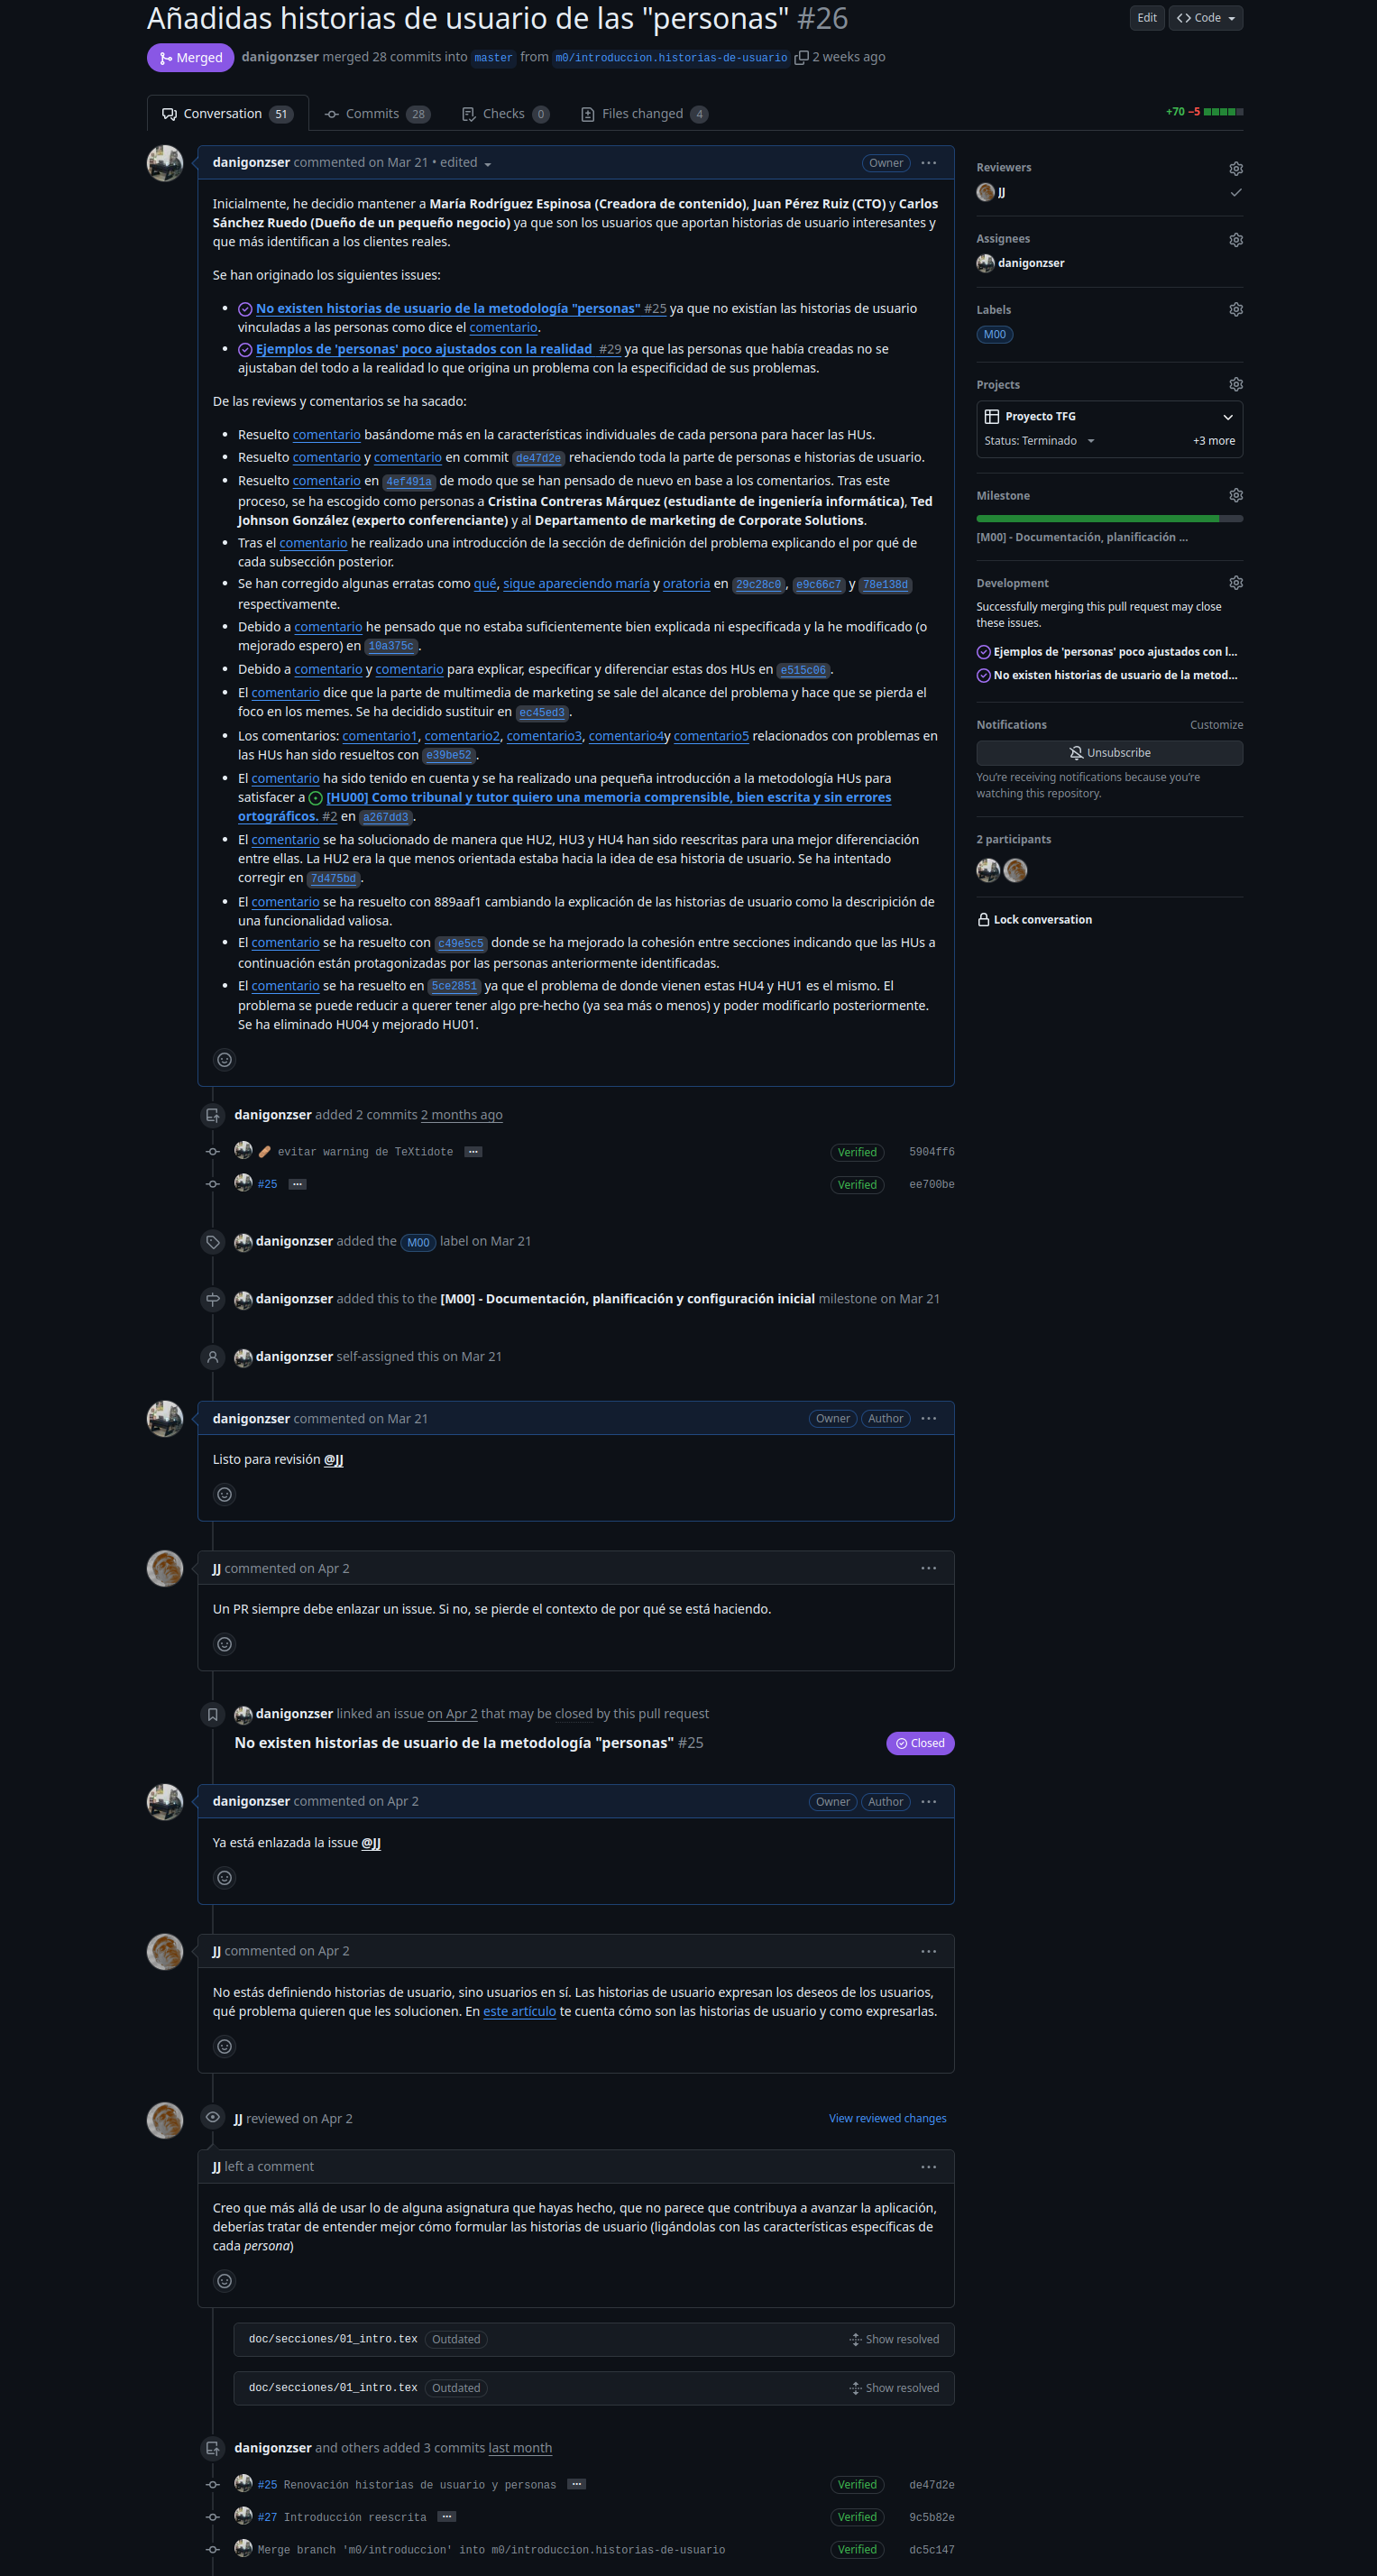
\includegraphics[scale=0.1]{figuras/pull_request_github.png}\label{fig:contenido_pull_request}
\end{figure}

Como se puede ver en la figura~\ref{fig:contenido_pull_request} el estado de la \textit{pull request} es \textit{merged} lo que significa que ya ha sido integrado en la rama principal. Más abajo se puede ver el cuerpo de la misma donde residen todas las \textit{issues} que han sido creadas y consecuentemente resueltas con esta \textit{pull request}. Más abajo se puede ver el historial de commits y de conversaciones que se han ido originando a lo largo de la resolución. Al final de la imagen es donde podemos ver esas conversaciones que deben ser resueltas antes de integrar los cambios en la rama principal. Finalmente, a la derecha se muestran detalles como el revisor, el asignado, las etiquetas, el proyecto al que pertenece, el \textit{milestone} y las \textit{issues} relacionadas.

\subsubsection{\textit{Projects}: tablero kanban}

La funcionalidad de projects de \textit{GitHub} se ha utilizado para llevar un control de la evolución y progreso de los \textit{issues} y \textit{pull requests}. Se ha implementado un tablero \textit{kanban} como se puede ver en la imagen~\ref{fig:tablero_kanban} que permite ver de un vistazo el estado de los \textit{issues} y \textit{pull requests}. Esto es muy útil para saber si se progresa, cómo se están resolviendo los problemas y si se está cumpliendo con los objetivos marcados. Además, está relacionado con los principios ágiles al promover la auto-organización, entrega frecuente y temprana y atención continua.

\begin{figure}[H]
    \caption{Captura de pantalla del tablero \textit{kanban} en la sección de \textit{projects} de \textit{GitHub}.}
    \centering
    \vspace*{0.5cm}
    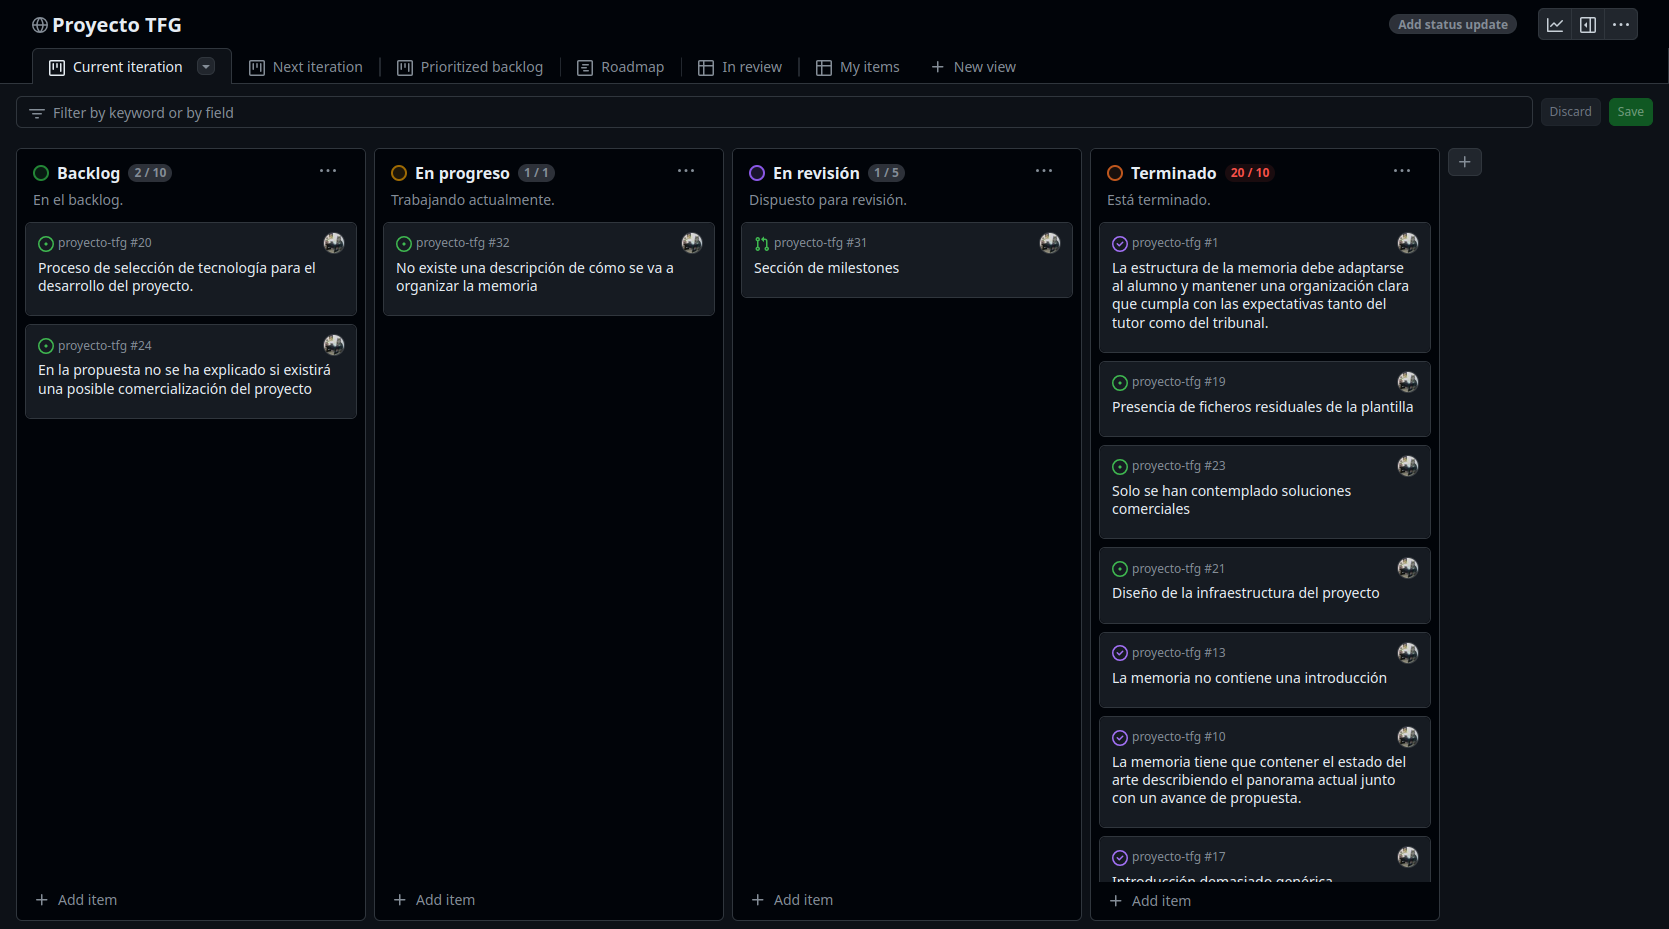
\includegraphics[scale=0.2]{figuras/projects_github.png}\label{fig:tablero_kanban}
\end{figure}

\section{Temporización}

La gestión de tiempo y recursos en nuestro proyecto se realiza mediante el uso de \textit{milestones} en GitHub, que son el equivalente a los \textit{sprints} en el enfoque ágil. Los \textit{milestones} se han creado a partir de las historias de usuario, asegurando que cada fase del proyecto esté orientada a cumplir con las necesidades y expectativas del usuario final. Un conjunto específico de \textit{issues} puede ser incluido en un \textit{milestone} y, al finalizar el \textit{sprint}, estos \textit{issues} deben estar resueltos. Al concluir el \textit{milestone}, debe resultar en un producto mínimamente viable y en nuestro repositorio vamos a etiquetarlos como nueva versión del proyecto.

\subsection{Milestones}

\begin{itemize}
    \item \textbf{[M00] \- Documentación, planificación y configuración inicial}
    \begin{itemize}
        \item \textit{Descripción}: Este \textit{milestone} abarca la creación de la documentación inicial, la planificación del proyecto y la configuración de las herramientas necesarias.
    \end{itemize}

    \item \textbf{[M01] \- Domain Driven Design}
    \begin{itemize}
        \item \textit{Descripción}: Enfocado en la implementación del diseño dirigido por el dominio (DDD).
    \end{itemize}
\end{itemize}

A partir de aquí, los \textit{milestones} se irán definiendo y ajustando conforme avance el proyecto, siguiendo los principios del desarrollo ágil que promueven la adaptación continua y la respuesta al cambio. Los \textit{milestones} sucesivos se centrarán en la implementación.

	% Análisis del problema
	% 1. Análisis de requisitos
	% 2. Análisis de las soluciones
	% 3. Solucion propuesta
	% 4. Análisis de seguridad
	\chapter{Análisis del problema}
 
\section{Análisis de las soluciones}

\section{Solucion propuesta}

\section{Análisis de seguridad}

	% Desarrollo bajo sprints: 
	% 	1. Permitir registros y login de usuarios
	% 	2. Desarrollo del sistema de incidencias
	% 	3. Desarrollo del sistema de denuncias administrativas y accidentes
	% 	4. Desarrollo del sistema de croquis
	%   5. Instalación de la aplicación de manera automática
	\chapter{Implementación}

La implementación del software se ha dividido en hitos. Estos, han sido definidos en Github
y cada uno de ellos contiene un grupo de \textit{issues} que se corresponden con las distintas
mejoras que se han ido incorporando al software a lo largo de su desarrollo.\\



	% Presupuesto

	\cite{gplv3}

	% Conclusiones
	\chapter{Conclusiones y trabajos futuros}



	% Trabajos futuros
	
	\newpage
	\bibliography{bibliografia}
	\bibliographystyle{plain}
	
\end{document}

